\chapter{Results \& Analysis}
\label{ch:res}
The models described in the previous section are simulated in \cite{cfx}. Note, refer to \hyperlink{appendixa}{Appendix A} for all plotted results.

%-----------------------------------------------------------------------------------------------------------------
\section{Convergence}
\label{sec:convg}

Monitoring of residuals $\delta_{r_{MAX}}$ is completed for all simulations to determine model performance (see Figures~\ref{fig:ref_convg}, \ref{fig:mod1_convg}, \ref{fig:mod2_convg}).

\begin{figure}[H]
	\centering
	\includegraphics[height=0.425\textheight,keepaspectratio]{ref/convergence}
	\caption{Reference model convergence.}
	\label{fig:ref_convg}
\end{figure}
\begin{figure}[H]
	\centering
	\includegraphics[height=0.425\textheight,keepaspectratio]{model1/convergence}
	\caption{Model 1 convergence.}
	\label{fig:mod1_convg}
\end{figure}
\begin{figure}[H]
	\centering
	\includegraphics[height=0.425\textheight,keepaspectratio]{model2/convergence}
	\caption{Model 2 convergence.}
	\label{fig:mod2_convg}
\end{figure}

Summarizing the above, models converged on $i_{ref}=39$, $i_1=36$, and $i_2=44$ iterations for the reference, model 1 and model 2, respectively. It is also clear that converge for reference and model 1 are smooth (see Figures~\ref{fig:ref_convg}, \ref{fig:mod1_convg}). Meanwhile, model 2  has some very small high frequency oscillations (see Figure~\ref{fig:mod2_convg}). This could be a result of opposing side inlet entrance velocity relative to the axial inlet.

%-----------------------------------------------------------------------------------------------------------------
\section{Validation}
\label{sec:valid}
The reference model is validated by comparing the CFX results to experimental data from \cite{art}. Velocity $u-v$ and turbulent KE $k$ data collected at $X^*=-0.87,\ 0,\ 1.6,\ 2.5,\ 4,\ 9$ are compared in the following plots.\\

Both simulated and experimental $u-v$ and $k$ profiles at various $X^*$ are shown below in Figure~\ref{fig:exp_ref_u}, \ref{fig:exp_ref_v}, \ref{fig:exp_ref_k}. Note, see \hyperlink{appendixb}{Appendix B} for \cite{matlab} script used to create all of the foregoing plots.\\
\begin{figure}[H]
	\centering
	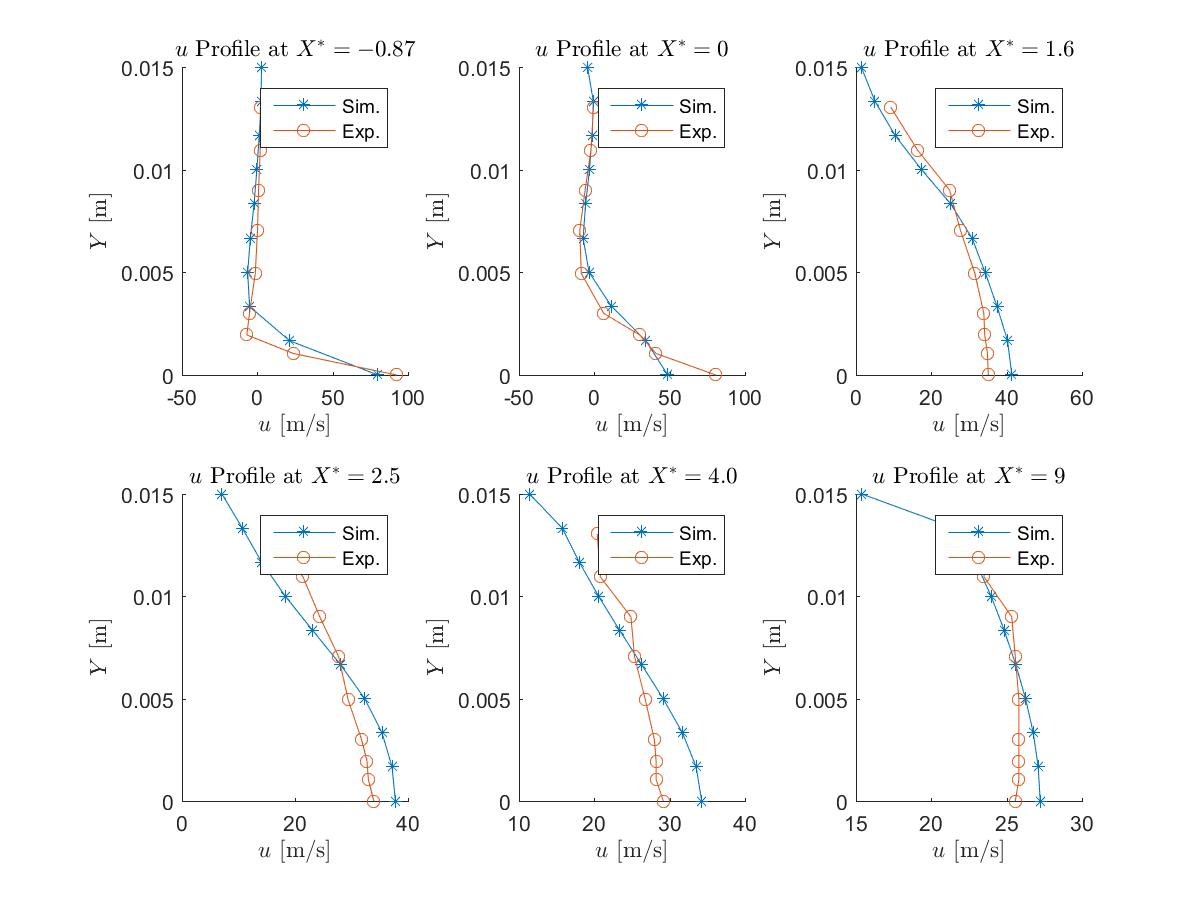
\includegraphics[height=0.425\textheight,keepaspectratio]{matlab/exp_ref_u}
	\caption{Comparison of experimental and simulated $u$ profiles at various $X^*$.}
	\label{fig:exp_ref_u}
\end{figure}

\begin{figure}[H]
	\centering
	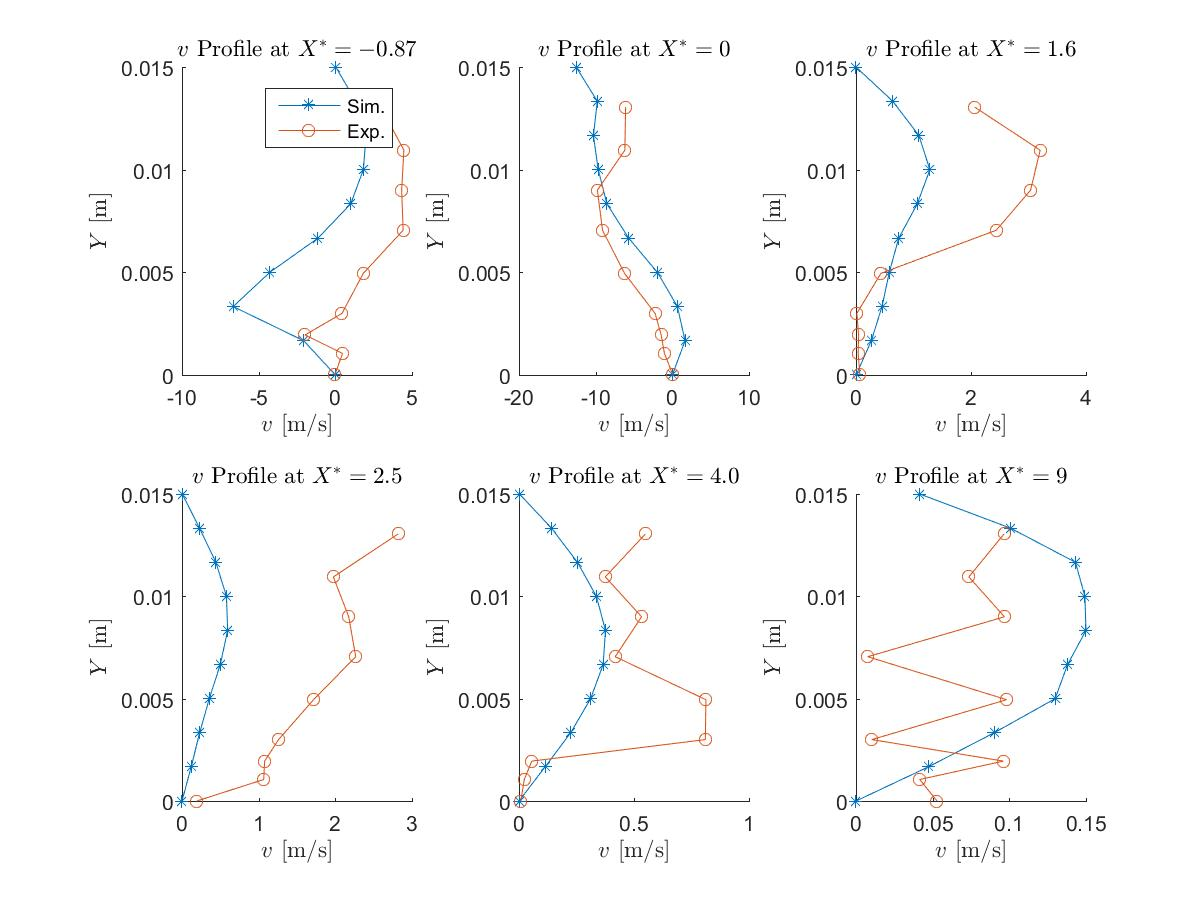
\includegraphics[height=0.425\textheight,keepaspectratio]{matlab/exp_ref_v}
	\caption{Comparison of experimental and simulated $v$ profiles at various $X^*$.}
	\label{fig:exp_ref_v}
\end{figure}

\begin{figure}[H]
	\centering
	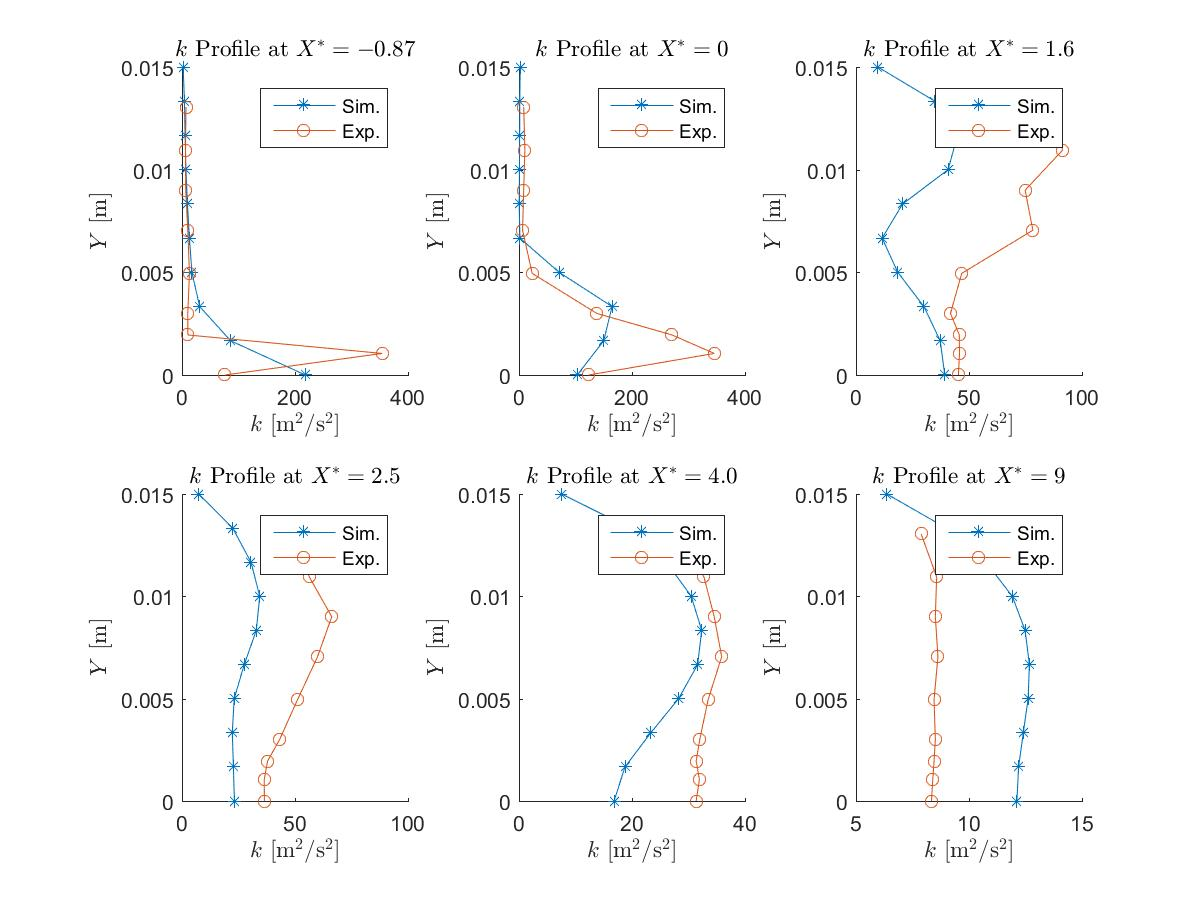
\includegraphics[height=0.425\textheight,keepaspectratio]{matlab/exp_ref_k}
	\caption{Comparison of experimental and simulated $k$ profiles at various $X^*$.}
	\label{fig:exp_ref_k}
\end{figure}

The simulated $u$ profiles match very well with experimental data for low $X^*$ (see Figure  \ref{fig:exp_ref_u}). Near the end of the domain, it appears that the discrepancies between data are larger.\\

As for both $v$ and $k$ profiles (Figures \ref{fig:exp_ref_v} and \ref{fig:exp_ref_k}) the simulation data does not compare very well with that of \cite{art}. Possible causes for these differences could be sources of errors which are described further in Section \ref{sec:err}. Furthermore experimental measurement error is also highly likely. This clearly depicted in the $v$ profile at $X^*=9$ (see Figure~\ref{fig:exp_ref_v}).
%-----------------------------------------------------------------------------------------------------------------
\section{Effects of Side Inlets}
\label{sec:effects_side}
The direct effect of side inlet angle is investigated in this sections. Velocity, turbulent KE and temperature profiles are extrapolated from 3D data in \hyperlink{appendixa}{Appendix A}.\\

Simulated $u$, $v$ and $k$ profiles for all models at various $X^*$ are shown below in Figures~\ref{fig:sim_compu} to \ref{fig:sim_compk}, respectively.
\begin{figure}[H]
	\centering
	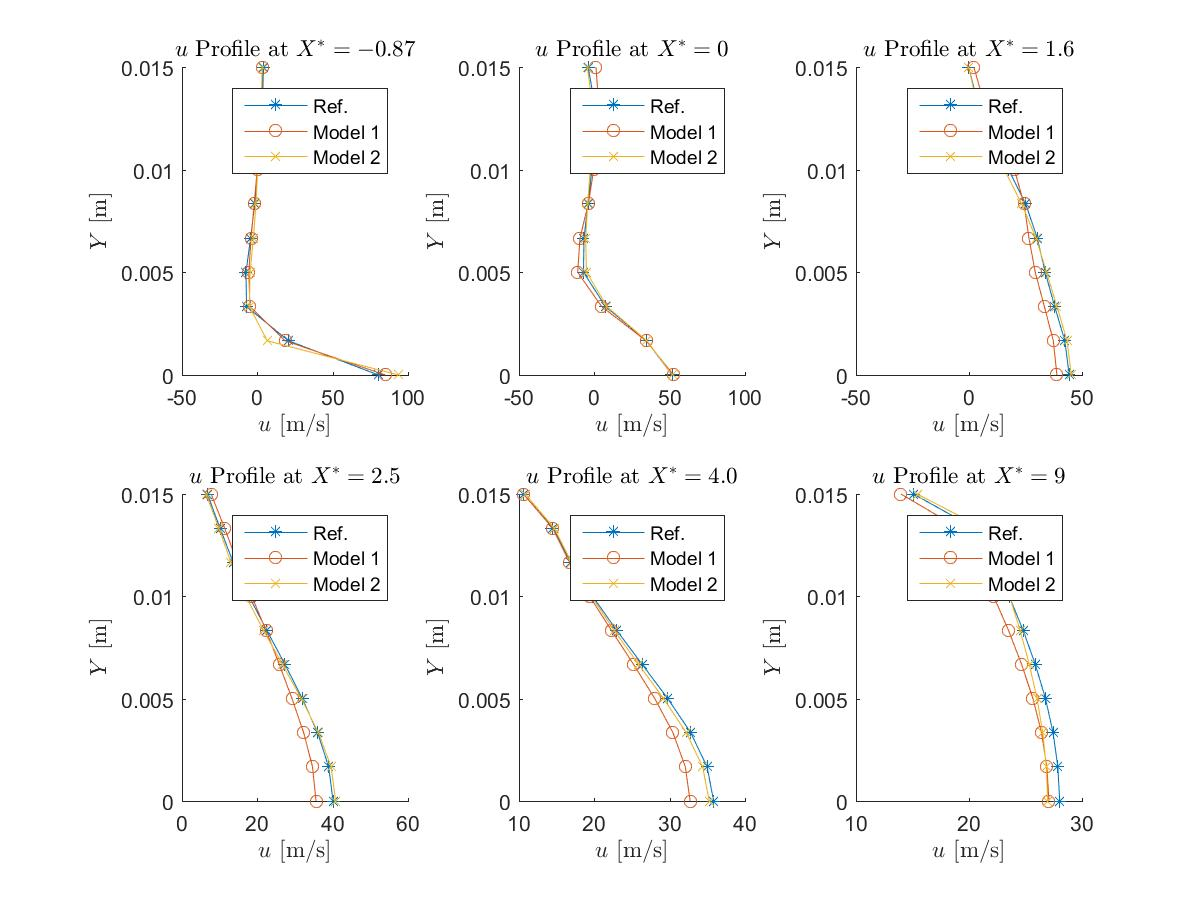
\includegraphics[height=0.425\textheight,keepaspectratio]{matlab/sim_compu}
	\caption{Comparison of all simulated $u$ profiles at various $X^*$.}
	\label{fig:sim_compu}
\end{figure}

\begin{figure}[H]
	\centering
	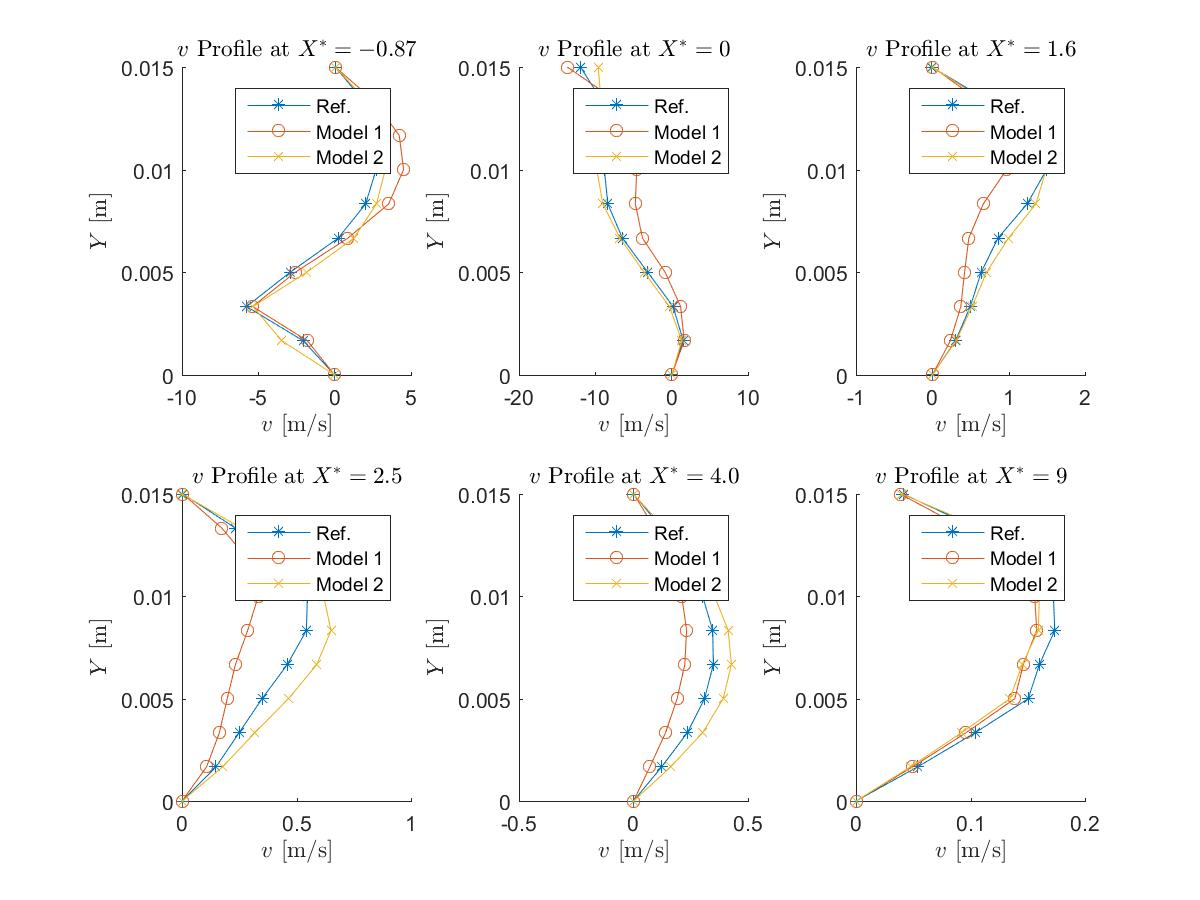
\includegraphics[height=0.425\textheight,keepaspectratio]{matlab/sim_compv}
	\caption{Comparison of all simulated $v$ profiles at various $X^*$.}
	\label{fig:sim_compv}
\end{figure}

\begin{figure}[H]
	\centering
	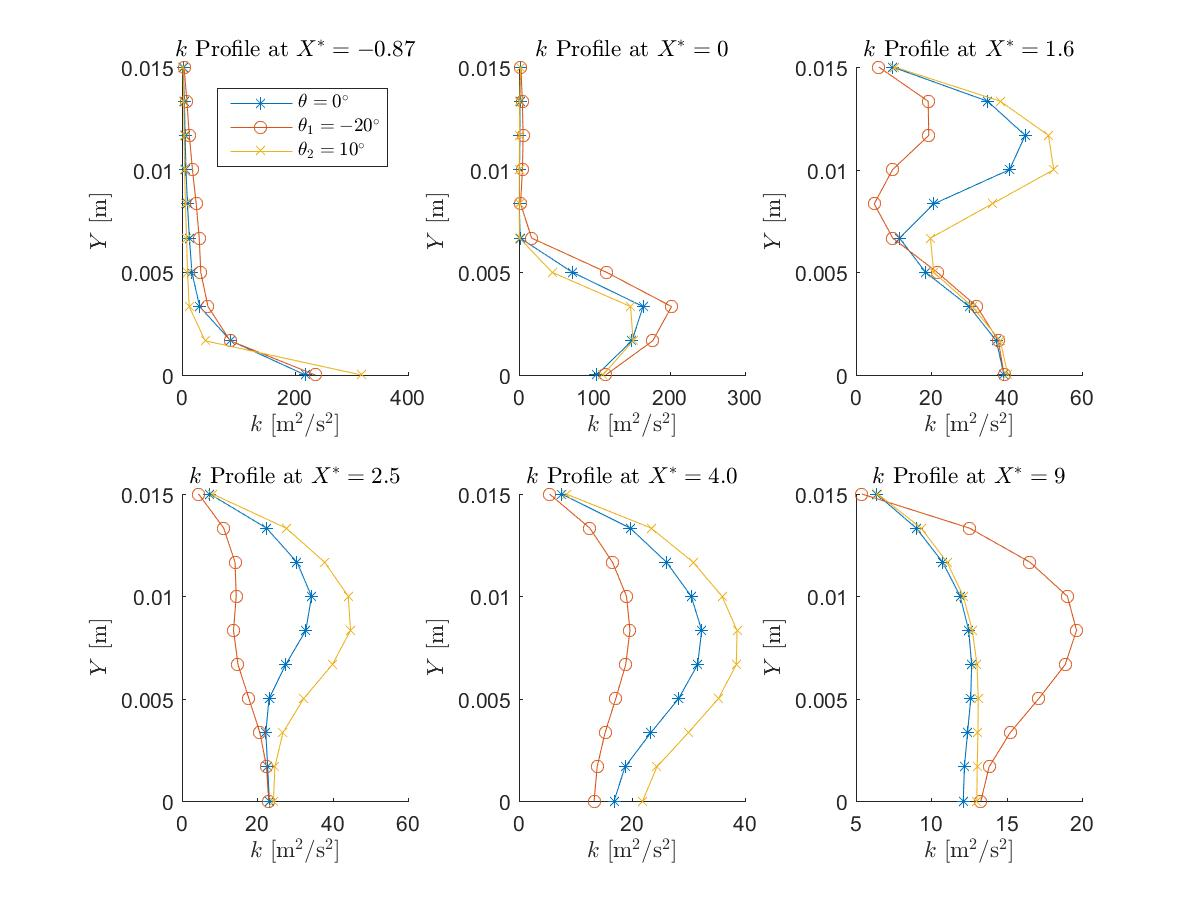
\includegraphics[height=0.425\textheight,keepaspectratio]{matlab/sim_compk}
	\caption{Comparison of all simulated $k$ profiles at various $X^*$.}
	\label{fig:sim_compk}
\end{figure}

Based on results from Figure \ref{fig:sim_compu}, there is hardly any variation in simulated $u$ profiles.\\

In Figures \ref{fig:sim_compv} and \ref{fig:sim_compk}, minimal variation is seen in both $v$ and $k$ profiles for $X^* \leq 0$ however, larger discrepancies are observed as $X^* \rightarrow 9$.\\

From the above plots, no clear distinction can be made between the results for each model. In hopes to better characterize the combustor's mixing ability, temperature $T$ profiles are shown in Figure \ref{fig:sim_compT} below.
\begin{figure}[H]
	\centering
	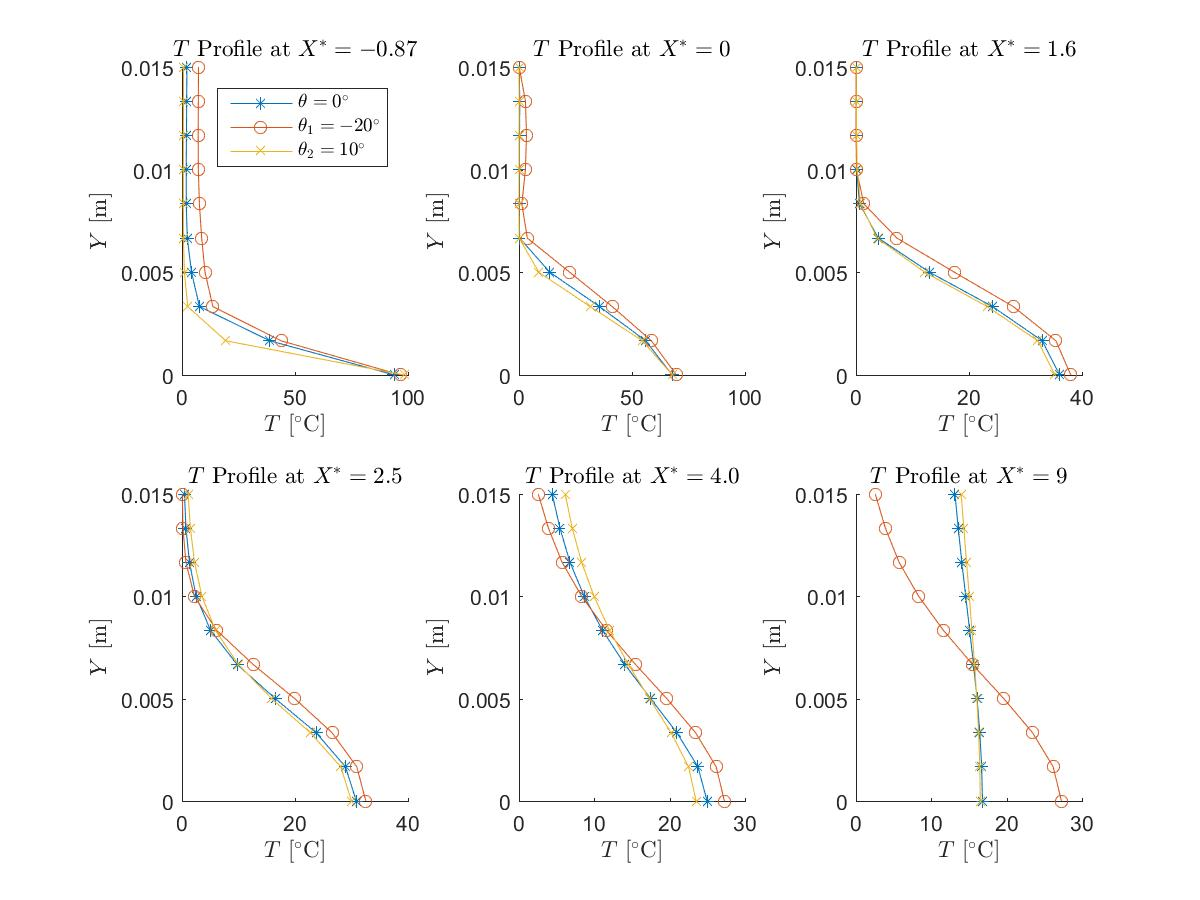
\includegraphics[height=0.425\textheight,keepaspectratio]{matlab/sim_compT}
	\caption{Comparison of all simulated $T$ profiles at various $X^*$.}
	\label{fig:sim_compT}
\end{figure}

Again, only a slight variation is observed in temperature profiles. This is also depicted graphically  in Figures \ref{fig:temp_ref} to \ref{fig:temp_mod2} in \hyperlink{appendixa}{Appendix A}.\\

Observations from above are further investigated below in Figures~\ref{fig:sim2_comp_T} and \ref{fig:sim2_comp_k} where $T$ and $k$ are plotted along $X^*$ at $Y^*=0$.

\begin{figure}[H]
	\centering
	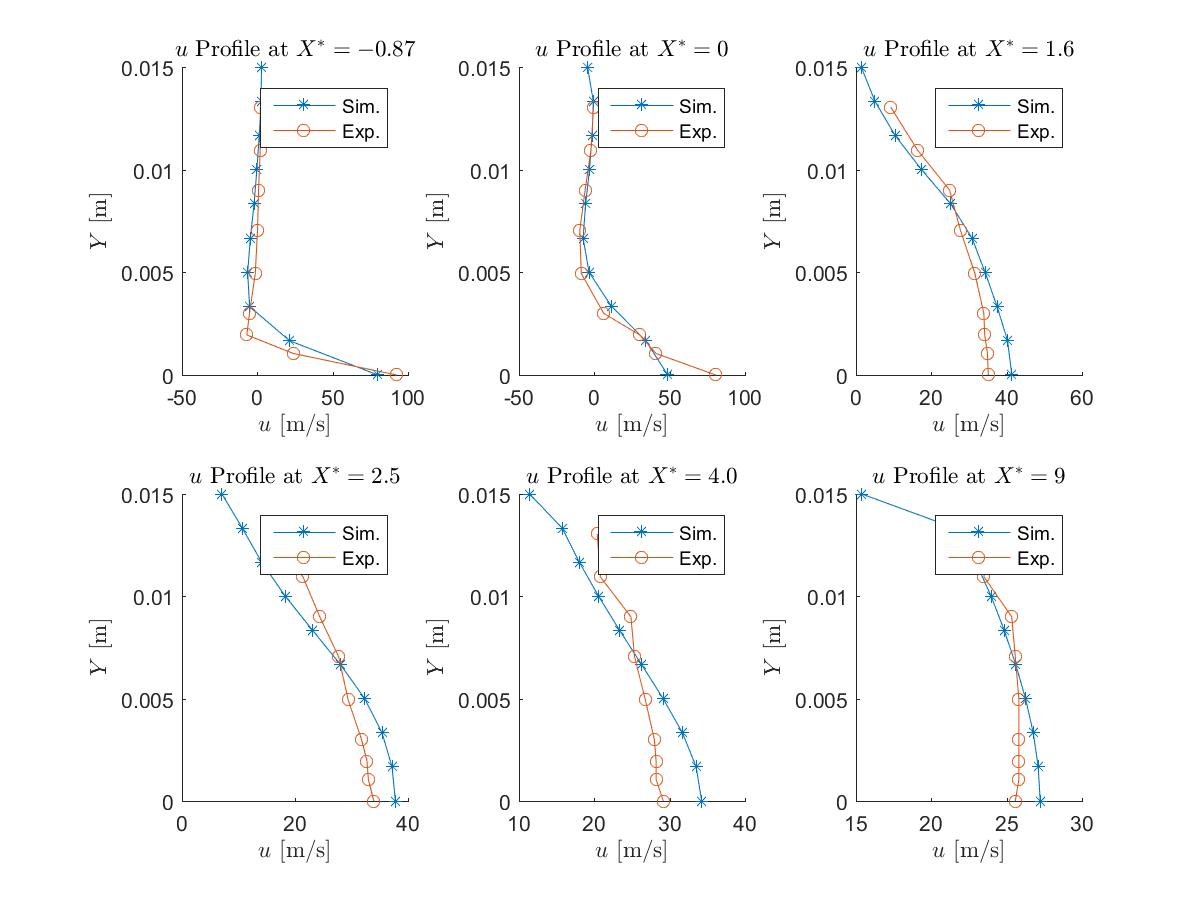
\includegraphics[height=0.425\textheight,keepaspectratio]{matlab/sim2_comp_T}
	\caption{Variation of $T$ along $X^*$ at $Y^*=0$.}
	\label{fig:sim2_comp_T}
\end{figure}

\begin{figure}[H]
	\centering
	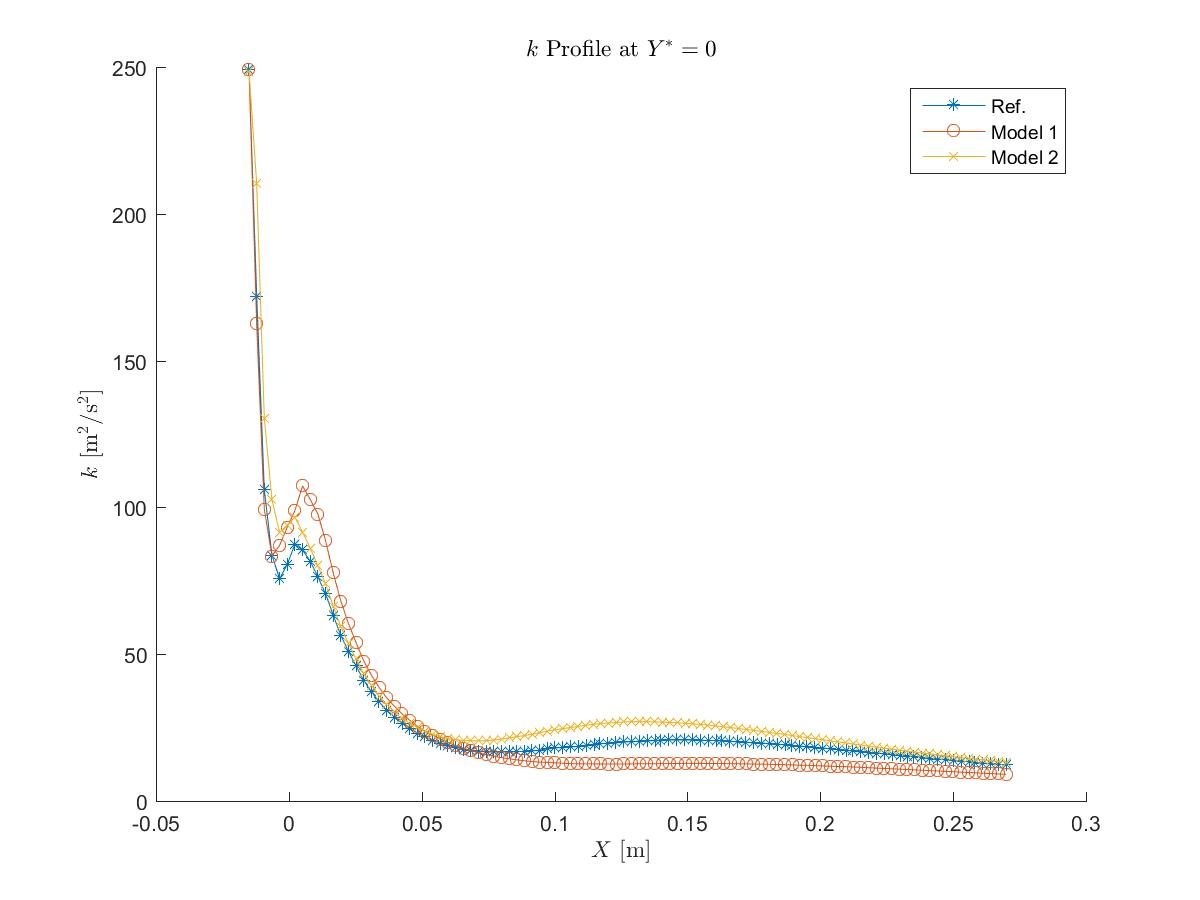
\includegraphics[height=0.425\textheight,keepaspectratio]{matlab/sim2_comp_k}
	\caption{Variation of $k$ along $X^*$ at $Y^*=0$.}
	\label{fig:sim2_comp_k}
\end{figure}

Axially, it appears as though a CCW angle of 20\textsuperscript{o} shows a slightly higher temperature as $X^* \rightarrow 9$ indicating the best mixing of all three models. This conclusion can also be explained through the variation of turbulent KE $k$ in Figure~\ref{fig:sim2_comp_k}. It can be observed that for model 2 ($\theta_2$), $k$ is higher near the entrance ($\approx X\leq 0.05$ [m] )and as $X\rightarrow 0.285$ [m], it can be seen that $k_1 < k_{ref} < k_2$. This states that initially, there is more turbulence in the domain but near the outlet, less disorder is observed hence indicating uniform mixing.
%-----------------------------------------------------------------------------------------------------------------
\section{Comparison}
\label{sec:comp}

From \cite{mobin}, optimal mixing was observed for a CW angle of 20\textsuperscript{o}. The same conclusion was reached by \cite{curtis} who saw a more uniform temperature mix for 10\textsuperscript{o} CW. Similarly to results in this report, best mixing was observed for a CCW angle of 10\textsuperscript{o} \cite{tolu}. Again, in \cite{study}, for a study of three large CCW angles,  30\textsuperscript{o} was deemed as the most uniform mixing. Possibilities for such discrepancies could be a result of differences in CFX-Pre models or errors which are discussed in the following section.
 
%-----------------------------------------------------------------------------------------------------------------
\section{Source of Errors}
\label{sec:err}

As with many CFD simulations, there is a plethora of error which must be considered and understood. Errors in the physical modelling from selected geometry, equations of state and turbulence model, will all effect the final solution in different ways. In these CFX simulations, the majority of the error is likely associated in the turbulence model. Justification for selection of the $k-\varepsilon$ turbulence model and its applicability was completed in Section \ref{sec:pre_fluid}. The pitfalls of this model is that it does not predict rotating flows very well \cite{cfdbook}. This is observed in Figures \ref{fig:velz_ref} to \ref{fig:velz_mod2} in \hyperlink{appendixa}{Appendix A}. To mitigate this source of error, a more powerful turbulence model such the large eddy simulation could be used as it models only smaller scales \cite{cfdbook}.\\

Furthermore, the numerical models also play a large role in error, primairly through discretization. For example, even though a high resolution scheme is selected due to its high accuracy in CFX, it is still only second order accurate or $\mathcal{O} (\Delta x^2)$ \cite{cfdbook}. Based on a node limit of approximately 20000 \cite{proj}, the minimum element size of 1 [mm] will cause some discretization error. This being said, the grid quality is considered to be poor due to this coarse mesh. Other sources of numerical error are also attributed to the computer's round off, truncation after each iteration as well as the final convergence criterion of the maximum specified residual.
